\documentclass[a4paper,11pt]{article}
\usepackage{cmap}
\usepackage{polski}
\usepackage[T1]{fontenc}
\usepackage[utf8]{inputenc}
\usepackage{listings}
\usepackage{graphicx}  
\graphicspath{ {C:/Users/jankl/} }



\title{Sprawozdanie nr 3}
\author{Łukasz Szumilas}
\date{Zajęcia: 19 listopad 2018}

\begin{document}
  \begin{center}\Large
    Grafika Komputerowa i Komunikacja Człowiek-Komputer
  \end{center}
  \hrule
  {\let\newpage\relax\maketitle}
  \hrule


  \section{Omówienie tematu}
  Ćwiczenie miało za zadanie pokazać, jak przy pomocy funkcji biblioteki OpenGL z rozszerzeniem GLUT można zrealizować prostą interakcję, polegającą na sterowaniu ruchem obiektu i położeniem obserwatora w przestrzeni 3D. Do sterowania miała służyć mysz.
\\\indent By obiekt za pomocą interakcji z użytkownikiem przemieszczał się we wszystkich osiach należy zastosować rzutowanie perspektywiczne. W rzucie perspektywicznym proste rzutowania nie biegną równolegle do \textit{osi z}, dlatego obracanie obiektu wzdłuż niej da nam porządany efekt pokazania obrazu ze wszystkich stron. Trójwymiarowy obiekt zdefiniowany na płaszczyźnie prezentuje się wtedy o wiele lepiej.
\\\indent Stosując kilka zmian, które prezentuje \textbf{\textit{kod 1}}, widać różnicę w prezentacji obiektu między dwoma rodzajami rzutów, którą ukazuje nam \textbf{\textit{rysunek 1}}. 
\\\indent Mając do dyspozycji szereg zmiennych pozwalających definiować obserwatora, możemy ustawić parametry z tych widocznych na \textit{rysunku 1 \\(gluLookAt(0.0, 0.0, 10.0, 0.0, 0.0, 0.0, 1.0, 0.0, 0.0))} na te widoczne na \textit{\textbf{rysunku 2}\\(gluLookAt(3.0, 3.0, 10.0, 0.0, 0.0, 0.0, 1.0, 1.0, 0.0))}
\\\indent Po sprawdzeniu jak działa nowe rzutowanie, czas na interakcję z użytkownikiem. Przy pomocy odpowiedniej implementacji (\textbf{\textit{kod 2}}) można sprawić, by imryk poruszał się dzięki kliknięciu i poruszeniu myszki wokół \textit{osi y}.
\\\indent Po dodaniu podobnej funkcji jak w kodzie nr 2 \textit{(glRotatef)}, można sprawić, by przedmiot obracał się także wokół \textit{osi x}, a więc już we wszystkie strony. Dodatkowo odpowiednio zmieniając drugi parametr funkcji \textit{gluLookAt} i używając prawy przycisk myszy, można przybliżać lub oddalać obraz.  (\textbf{\textit{kod 3, rys3}}).
\\\indent Eksperymentować z rzutem można za pomocą dwóch sposobów. Pierwszym jest obracanie samego modelu. W drugim to obserwator przemieszcza się dokoła modelu. Sterowanie położeniem obserwatora odbywa się powinno przy pomocy dwóch kątów : \textbf{azymutu} i \textbf{elewacji}. Pierwszy z nich określa kierunek patrzenia na obiekt, drugi wysokość położenia obserwatora nad "horyzontem". Pod uwagę trzeba wziąć także promień, który określa oddalenie się obserwatora od obiektu. Pełen wzór na położenie obserwującego, ze strony zawierającej instrukcję laboratorium:
    \begin{figure}[h!]
      \centering
      \includegraphics[width=0.6\textwidth,height=3cm]{kodobserwatora.jpg}
      \label{fig:zrzut1}
    \end{figure} 
\\\indent Tym razem do zmiany położenia nie posłuży już funkcja \textit{glRotatef}. Skoro to obserwator ma być stroną czynną, zmiany będą zachodziły w  \textit{glLookAt}. Ważne jest, by pamiętać o ograniczeniach dotyczących obrotów i przybliżania. Zoom nie może powiększać się w nieskończoność, spowodowałoby to "przeskoczenie" na drugą stronę obiektu, co zmniejszyłoby realistykę interakcji. Tak samo kąt azymutu i elewacji nie może się zmieniać cały czas. Po odpowiednim obrocie musi nastąpić wyzerowanie kąta, inaczej hipotetyczna kamera trzymana przez obserwatora wprowadzi niepożądane zmiany w położeniu. Pełen kod i zrzut ekranu obrazujący efekty implementacji widnieje w  \textit{\textbf{kodzie nr 4, rysunku 4}}. Przy obracaniu się obserwatora dobrze widoczna jest zmiana położenia \textit{osi z}, dając lepsze wrażenie ingerencji jedynie w ruch wokół, a nie samego modelu. 

  \section{Omówienie kodu}
   \textbf{Kod 1}, funkcja użyta w innej, już znanej funkcji, \textit{RenderScene()}, pozwalająca zdefiniować hipotetycznego obserwatora. 
\\\indent W funkcji \textit{ChangeSize()}  natomiast w miejsce \textit{glOrtho()} użyto funkcję \textit{gluPerspective(}), która służy do definiowania obszaru widoczności dla rzutu perspektywicznego.
{\small
\begin{lstlisting}[language=C++]

void gluLookAt(GLdouble eyeX, GLdouble eyeY, GLdouble eyeZ,                                 
   //miejsce, w ktorym stoi obserwator
GLdouble centerX, GLdouble centerY, GLdouble centerZ,            
//punkt, na ktory obserwator patrzy
 GLdouble upX , GLdouble upY, GLdouble upZ);		        
 //polozenie kamery trzymanej przez obserwatora,
 "przechyla" obraz w jedna badz druga strone

}

void gluPerspective(GLdouble fovy, GLdouble aspect, 
GLdouble zNear, GLdouble zFar)
\end{lstlisting}
}
.\\
\textbf{Kod 2} pomoże w prostej iterakcji z użytkownikiem, dzięki której będzie mógł obracać dany obiekt.
{\small
\begin{lstlisting}[language=C++]
//zmienne globalne
static GLfloat theta = 0.0;   
// kat obrotu obiektu
static GLfloat pix2angle;    
 // przelicznik pikseli na stopnie

static GLint status = 0;      
 // stan klawiszy myszy 
                            
   // 0 - nie nacisnieto zadnego klawisza
   // 1 - nacisniety zostal lewy klawisz

static int x_pos_old=0;      
 // poprzednia pozycja kursora myszy

static int delta_x = 0;       
 // roznica pomiedzy pozycja biezaca
// i poprzednia kursora myszy 


// Funkcja sprawdza stan myszy 
//i ustawia wartosci odpowiednich zmiennych globalnych

void Mouse(int btn, int state, int x, int y)
{
  if(btn==GLUT_LEFT_BUTTON && state == GLUT_DOWN)        
    {
 x_pos_old=x;         
// przypisanie aktualnie odczytanej pozycji kursora 
// jako pozycji poprzedniej
status = 1;         
 // wcisniety zostal lewy klawisz myszy
    } 
  else
  status = 0;          
// nie zostal wcisniety zaden klawisz 
}

// Funkcja sprawdza polozenie kursora myszy
// i ustawia wartosci odpowiednich zmiennych globalnych

void Motion( GLsizei x, GLsizei y )
{
 delta_x=x-x_pos_old;    
 // obliczenie roznicy polozenia kursora myszy
  x_pos_old=x;           
 // podstawienie biezacego polozenia jako poprzednie
  glutPostRedisplay();     
// przerysowanie obrazu sceny
}

//w main()
glutMouseFunc(Mouse);
// Ustala funkcje zwrotna odpowiedzialna za badanie stanu myszy
    
glutMotionFunc(Motion);
// Ustala funkcje zwrotna odpowiedzialna za badanie ruchu myszy


//linia w funkcji ChangeSize()
pix2angle = 360.0/(float)horizontal;  
// przeliczenie pikseli na stopnie


//linie w funkcji RenderScene() przed tworzeniem imbryka
if(status == 1)             
{
   theta += delta_x*pix2angle;   
 // modyfikacja kata obrotu
}                                 

glRotatef(theta, 0.0, 1.0, 0.0); 
 //obrot obiektu o nowy kat
\end{lstlisting}
}

.\\
\textbf{Kod 3}, analogicznie jak w stosunku do osi y.   
{\small
\begin{lstlisting}[language=C++]
//globalne
static GLint status1 = 0
static int y_pos_old = 0;      
static int delta_y = 0;

//dodanie ponizszych linijek w funkcji Mouse()
if (btn == GLUT_LEFT_BUTTON && state == GLUT_DOWN)
{
y_pos_old = y;
status = 1;
}
else if (btn == GLUT_RIGHT_BUTTON && state == GLUT_DOWN)
{
status1 = 1;
}

//dodanie ponizszych linijek w funkcji Motion()
delta_y = y - y_pos_old;
y_pos_old = y;

//przy zmianie statusu przycisku w RenderScene()
if (status == 1)              
{
theta1 += delta_y * pix2angle;
}
if (status1 == 1)  
{
viewer[2] += (delta_y*0.1); //zoom
}
glRotatef(theta1, 1.0, 0.0, 0.0);
\end{lstlisting}
}
.\\
\textbf{Kod 4}, pełen kod definiujący położenie obserwatora i możność jego zmian
{\small
\begin{lstlisting}[language=C++]

#include <Windows.h>
#include <GL\glew.h>
#include <GL\freeglut.h>
#include <iostream>
#include <cmath>

using namespace std;

typedef float point3[3];

static GLfloat azymut = 0;
static GLfloat elewacja = 0;
static GLfloat R = 10;
static GLfloat Vy = 1;

static GLfloat x = R * cos(azymut) * cos(elewacja);
static GLfloat y = R * sin(elewacja);
static GLfloat z = R * sin(azymut) * cos(elewacja);

static GLfloat viewer[] = { x, y, z };

static GLfloat theta = 0.0;   
static GLfloat theta1 = 0.0;
static GLfloat pix2angle;   
static GLfloat angle2rad;    

static GLint status = 0;       
static GLint status1 = 0; 	  
							 

static int x_pos_old = 0;      
static int y_pos_old = 0;       

static int delta_x = 0;       
static int delta_y = 0;

void Axes(void)
{

point3  x_min = { -5.0, 0.0, 0.0 };
point3  x_max = { 5.0, 0.0, 0.0 };


point3  y_min = { 0.0, -5.0, 0.0 };
point3  y_max = { 0.0,  5.0, 0.0 };
point3  z_min = { 0.0, 0.0, -5.0 };
point3  z_max = { 0.0, 0.0,  5.0 };

glColor3f(1.0f, 0.0f, 0.0f);
glBegin(GL_LINES);
glVertex3fv(x_min);
glVertex3fv(x_max);
glEnd();

glColor3f(0.0f, 1.0f, 0.0f);
glBegin(GL_LINES);

glVertex3fv(y_min);
glVertex3fv(y_max);
glEnd();

glColor3f(0.0f, 0.0f, 1.0f);
glBegin(GL_LINES);

glVertex3fv(z_min);
glVertex3fv(z_max);
glEnd();
}


void Mouse(int btn, int state, int x, int y)
{
if (btn == GLUT_LEFT_BUTTON && state == GLUT_DOWN)
{
x_pos_old = x; 
y_pos_old = y;
status = 1;
}

else if (btn == GLUT_RIGHT_BUTTON && state == GLUT_DOWN)
{
status1 = 1;
}

else
{
status = 0;       
status1 = 0;
}
}

void Motion(GLsizei x, GLsizei y)
{
delta_x = x - x_pos_old;    
delta_y = y - y_pos_old;
x_pos_old = x;       
y_pos_old = y;

glutPostRedisplay();    
}


void RenderScene(void)
{
glClear(GL_COLOR_BUFFER_BIT | GL_DEPTH_BUFFER_BIT);

glLoadIdentity();

gluLookAt(viewer[0], viewer[1], viewer[2], 0.0, 0.0, 0.0, 0.0, Vy, 0.0);

Axes();

if (status == 1)
{
theta += delta_x * pix2angle;
theta1 += delta_y * pix2angle;
azymut = theta * angle2rad;
elewacja = theta1 * angle2rad;

if (azymut <= 0) azymut += 2 * 3.141592;
if (elewacja <= 0) elewacja += 2 * 3.141592;
if (azymut > 2 * 3.141592) azymut -= 2 * 3.141592;
if (elewacja > 2 * 3.141592) elewacja -= 2 * 3.141592;

if ((elewacja < (1.5*3.141592)) && (elewacja > (0.5*3.141592)))
{
Vy = -1;
}
else Vy = 1;

x = R * cos(azymut) * cos(elewacja);
y = R * sin(elewacja);
z = R * sin(azymut) * cos(elewacja);
viewer[0] = x;
viewer[1] = y;
viewer[2] = z;

}

if (status1 == 1)
{
R += (delta_y*0.1);
if (R >= 20 || R <= 2)
{
R -= (delta_y*0.1);
}
x = R * cos(azymut) * cos(elewacja);
y = R * sin(elewacja);
z = R * sin(azymut) * cos(elewacja);
viewer[0] = x;
viewer[1] = y;
viewer[2] = z;

	}

glColor3f(1.0f, 1.0f, 1.0f);

glutWireTeapot(3.0);
glFlush();
glutSwapBuffers();


}


void MyInit(void)
{
glClearColor(0.0f, 0.0f, 0.0f, 1.0f);
}


void ChangeSize(GLsizei horizontal, GLsizei vertical)
{
pix2angle = 360.0 / (float)horizontal;  
angle2rad = pix2angle * (3.141592 / 180.0);

glMatrixMode(GL_PROJECTION);

glLoadIdentity();

gluPerspective(70, 1.0, 1.0, 30.0);

if (horizontal <= vertical)
glViewport(0, (vertical - horizontal) / 2, 
	horizontal, horizontal);

else
glViewport((horizontal - vertical) / 2, 0, vertical, vertical);

glMatrixMode(GL_MODELVIEW);
glLoadIdentity();

}

int main(int argc, char* argv[])
{
glutInit(&argc, argv);

glutInitDisplayMode(GLUT_DOUBLE | GLUT_RGB | GLUT_DEPTH);

glutInitWindowSize(300, 300);

glutCreateWindow("Rzutowanie perspektywiczne");

glutMouseFunc(Mouse);
glutMotionFunc(Motion);

glutDisplayFunc(RenderScene);


glutReshapeFunc(ChangeSize);

MyInit();
glEnable(GL_DEPTH_TEST);

glutMainLoop();

system("pause");
return 0;
}
\end{lstlisting}
}



  \section{Rezultat prac}

    \begin{figure}[h!]
      \centering
      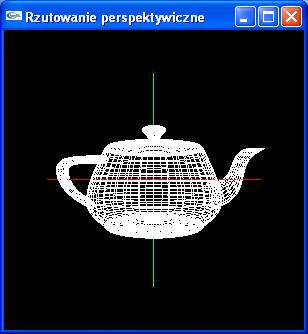
\includegraphics[width=0.6\textwidth,height=8cm]{rzutperspektywiczny.jpg}
      \caption{Imbryczek. Rzut perspektywiczny}
      \label{fig:zrzut1}
    \end{figure}

    \begin{figure}[h!]
      \centering
      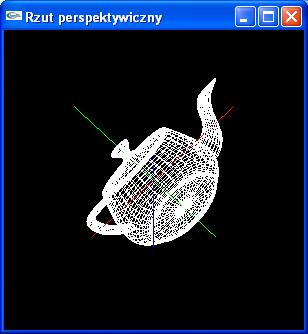
\includegraphics[width=0.6\textwidth,height=8cm]{rzutperspektywiczny1.jpg}
      \caption{Imbryczek po transformacji}
      \label{fig:zrzut1}
    \end{figure}

    \begin{figure}[h!]
      \centering
      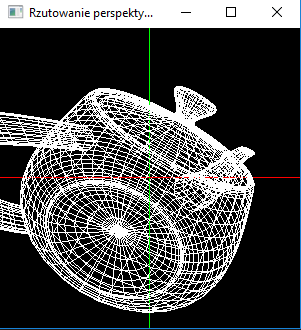
\includegraphics[width=0.6\textwidth,height=8cm]{obrotizoom.png}
      \caption{Obrót i zoom}
      \label{fig:zrzut1}
    \end{figure}

    \begin{figure}[h!]
      \centering
      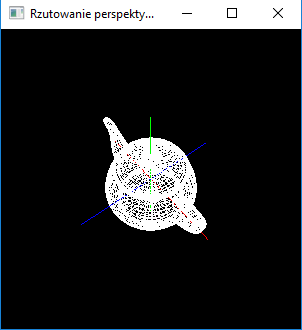
\includegraphics[width=0.6\textwidth,height=8cm]{ostatni.png}
      \caption{Obserwator stoi za imbrykiem, widzi go z góry i jest lekko oddalony}
      \label{fig:zrzut1}
    \end{figure}

\end{document}